\chapter{Approach}\label{ch:approach}
This PhD work adopts a socio-technical view towards the planning support systems in disaster response settings. Introducing a planning support system to \acf{DR} operations may create a socio-technical gap that needs to be considered by system designers. We argue that the gap can be reduced by an appropriate interaction design supported by a deep understanding of the socio-technical issues surrounding the planning support. In order to gain insight into the socio-technical issues, we adopted an ethnographic approach to explore and unpack interactions between humans and the planning support agent in a disaster setting. A serious \acf{MRG} approach is adopted to create the game \acf{AO}, which is used to simulate \ac{DR} operations. We outline two interaction designs that are later implemented in the \ac{AO} platform for field studies. In addition, efforts have been made to establish contact with a professional response agency, \acf{RG}, which took part in workshop centered on the \ac{AO} game. Feedback on \ac{AO} are collected from the discussions in the workshop. \\

In this chapter, we set out the socio-technical perspective to planning support systems adopted by this PhD work (section \ref{sec:sociotech} ), followed by an introduction to the serious \acf{MRG} approach (section \ref{sec:SMRG}) and description of AtomicOrchid platform (section \ref{sec:AOdescription}). The section \ref{sec:patterns} outlines the two interaction designs that are studied in the \ac{AO} field studies, and the section \ref{sec:rg} gives an introduction to the workshop with \ac{RG} for professional feedback. \\


\section{Adopting the socio-technical perspective}\label{sec:sociotech}
This research aims to inform the design of planning support for organizational work conducted by responder teams. This PhD work adopts a socio-technical view on the responder teams and their technological supporting systems. Integrating new technology support into a human organisation is a well-known challenge for socio-technical system design. In this PhD study, we anticipate the same challenges will be encountered when introducing a planning support system in disaster response operations.\\

The term socio-technical systems is used to describe systems that involve a complex interaction between humans, machines and the environmental aspects of the system (Section \ref{sec:LRSocialTechnical}). The term stands for the recognition of both technical and social subsystems and the very complex relationship between the two. Social systems are characterized by phenomena such as communication and cooperation between human individuals, emergence of meaning systems, self-referential development of structures. In contrast, technical systems are characterized by artefacts, control, anticipation, state-transitions, pre-programmed adaptability, learning in respect to purposes which are determined from outside the system \citep{Ropohl1999}. Introducing a technology support system into an organization requires the technical system and social aspects to be integrated.\\

In the context of this study, a multi-agent coordination algorithm is used to build an automated planning agent. From a technical point of view,  the planning agent requires a set of rigid inputs and produces plans of task allocations. For a fully autonomous system, plans can be handed over to other components for execution. Re-planning is usually triggered when an unanticipated situation happens. However the plan-execution model may be very different from the way that human make plans and take actions (Figure \ref{fig:gap}). For human teams, no matter how well the plan is formed, its significance in determining the actual actions is questionable. \ref{sec:LRSocialTechnical} showed that actions are highly dependent upon its material and social circumstances focusing on local interactions between actors, and environments of their action. Computer science is learning how to use techniques such as machine learning and user modelling to build agents with social capabilities (Section \ref{sec:LRHAI}). However, such attempts are still based on the approach of plan/intent recognition, which tries to establish logical links between human actions and intention.  It is hard to disprove that a technical solution is imminent, but many \ac{HCI} researchers have pointed out that it could be extremely difficult as the causal connections between actions and intent is weak (Section \ref{sec:LRSocialTechnical}). Arguably, the lack of causal links between intention, plan and actions makes human behaviours hard to predict and generalize from one situation to the next. Therefore, it is important to understand the specific organisational work and social processes in designing human system interactions that support, rather then hinder the social process of human teams. The aim of this thesis is to investigate specific social situations of \ac{DR} organisational work to inform interaction design of planning support systems. \\

\begin{figure}[H]
  \centering
  \rotatebox{90}{
  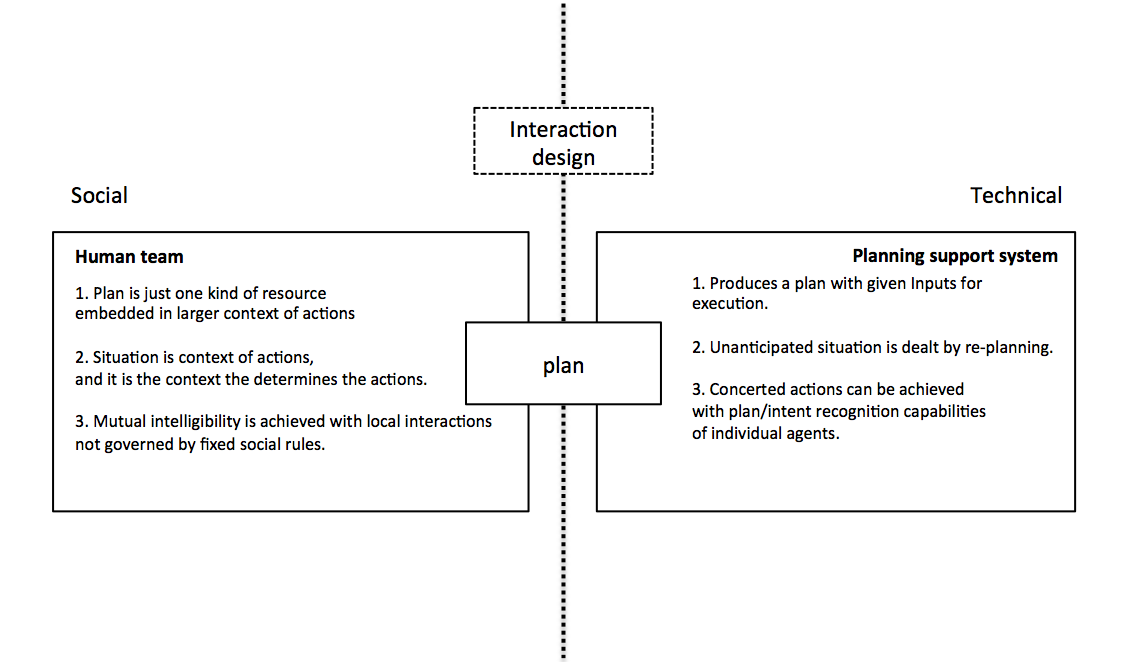
\includegraphics[width=1.5\textwidth]{img/approach/gap}
  }
  \caption{Actions and situated actions}
  \label{fig:gap}
\end{figure}

%On the other hand, planning activities of responder teams are characterized by natural social processes such as communication, negotiation and cooperation. To support the responder teams with multi-agent coordination technologies, the confrontation between social and technical is inevitable. \\

% Situated action and purposful action.

%\ac{CSCW} Researchers have pointed out the existence of the inherent social technical gap - the great divide between what we know we must support socially and what we can support technically.  Some argued that human activity is highly flexible, nuanced, and contextualized and that computational entities and processes such as information sharing, roles, and social norms need to be similarly flexible, nuanced, and contextualized. However, current technology support systems for organisations are often rigid and inflexible, failing to fully support the social world. 

%Computer science is learning how to use techniques such as machine learning, user modelling to fill social-technical gap (section \ref{sec:LRHAI}). It is hard to disprove that a technical solution is imminent. However, some argued that such a technical solution is unlikely, given that computer science, \acf{AI}, information technology, and information science researchers have attempted to bridge the gap without success for at least 20 years \cite{Ackerman2000}.\\

%We argue that the social aspect does not need to be fully supported through technological advance. A deep understanding of social issues and appropriate interaction design may lead to possible ``workaround'' of the socio-technical gap. Although technology support may be not fully integrated with the social aspects, we believe appropriate interaction design can reduce its negative impact on social process so that the benefits of technology can overweight its adverse social impact. \\

%The field of HCI achieved widespread recognition with its inherent focus on the importance of the interaction between people and technology at the fundamental level rather than just the design of the user interface. It explicitly recognised the importance of the roles of the social and technical aspects of work. HCI Literatures have identified a wide range of different methodologies that helps inform the development of socio-technical systems such as (1) Cognitive Work Analysis, (2) Ethnographic workplace analysis, (3) Human-centred design. Some of the recognised HCI methodologies underpin the serious game approach employed by this PhD work to understand socio-technical design space of agent-based planning support. [The switch to HCI is not smooth]\\

%[Field trials supported by interaction analysis  speech act]\\

%[Andy s literature review of 2004 supporting ethnographic study should be cited]\\


\section{Serious Mixed Reality Games as a testbed} \label{sec:SMRG}
One of our work`s main objectives is to study interaction and coordination situated in rich and `messy' real-world socio-technical settings. As it is difficult to deploy technological prototypes in real disasters, a serious game approach has been adopted by researchers to study technology interaction in disaster scenarios through game-like simulations (Section \ref{sec:LRMRgame}).
%for example, to prepare first responders for scenarios in which hazardous materials are involved \cite{Losh2007}. \cite{Abbasi2012} also presented a study in which locally distributed participants played the role of victims asking for help via social media in a simulated crisis, and participants that played the role of first responders used a coordination system to filter messages and mobilize the appropriate responder teams according to their assigned capabilities.\\

This PhD work also adopts serious game approach to simulate a disaster response setting in which distributed responder teams coordinate under temporal and spatial constraints (Section \ref{sec:LRtaskplanning}). More specifically, we create a \acf{MRG} as a testbed that enables studying team coordination, interaction and communication in a real-world disaster scenario whilst providing confidence in the efficacy of behavioural observations (Section \ref{sec:LRMRgame}).\\

The \ac{MRG} testbed called \acf{AO} simulates a radioactive incident. Participants of the game play both the role of responders `on the ground', and coordinators in the control room. They coordinate with each other through GPS, map sharing and messaging, to achieve game objectives. The \ac{AO} game system can be integrated with planning agents to support players on the ground, and the interaction layer between players and agents can be configured in different ways through modifications to the game interface. Through agent integration and interface modifications, we created three `probes' of agent planning support with different interaction designs. The three probes were then used to conduct observational studies, which allow us to unpack human system interaction in the different interaction design settings.\\

\section{The AtomicOrchid Platform}\label{sec:AOdescription}
We designed and implemented the mixed reality game \acf{AO} as a testbed for our field trials of different system interaction designs. The game involves field players on the ground (playing as field responders) and online players in a control room (playing as Headquarters (HQ)).

\begin{figure}[h]
  \centering
  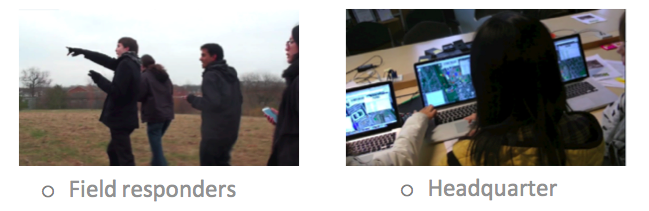
\includegraphics[width=1\textwidth]{img/approach/GameComponents}
  \caption{HQ and field players in AO}
  \label{fig:AOroles}
\end{figure}

In the following sections, we give a detailed description of the game design, which covers  grounding of the design rationale, the iterative design process, and the system architecture.

\subsection{Game mechanics} \label{sec:gameRatinale}
The AtomicOrchid is based on the fictitious scenario of a radioactive explosions creating expanding and moving radioactive clouds that pose a threat to responders on the ground (field responders), and the (virtual) targets to be rescued from around the game area. We chose a radiation scenario because unlike disasters that cause physical devastation it poses an invisible threat, which creates the need to monitor the environment closely with sensing devices, and communicate frequently.\\

Field responders are supported by a centrally located headquarters (HQ) control room, staffed by HQ players as coordinators who exchange messages with field players through an instant messaging style communication system. The messages are broadcasted, which means they are visible to all players. The core game mechanics are designed to allow us to explore specific aspects of team coordination. In particular, this is inspired by the real coordination challenge of resource and task allocation to coordinate spatially distributed resources and personnel. 

%The game`s two-tiered organisational structure is derived from real world disaster response organisation and from NIMS . The game`s HQ is loosely modelled on sector coordinators, whose role is to manage resources and communications between their assigned teams, and command and coordinate action within their sector (INSARAG, 2012). Field responders are modelled on team leaders and members. We ignore this distinction to simplify roles, assignments, and game mechanics.\\

%Whilst formal response teams tend to use radio to communicate (e.g., Toups et al., 2011) we chose text-based messages for its flexibility to support scenarios with many distributed (volunteer) field responders.\\

\textbf{Responder roles and targets}. Each field responder is assigned one of four roles:\\

\begin{figure}[h]
  \centering
  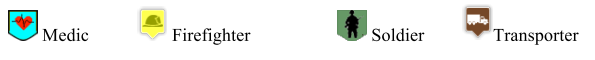
\includegraphics[width=1\textwidth]{img/approach/AOroles}
  \caption{The roles in \ac{AO}}
  \label{fig:AOroles}
\end{figure}

There are also four types of (virtual) targets:\\

\begin{figure}[h]
  \centering
  
\includegraphics[width=1\textwidth]{img/approach/AOtargets}
  \caption{The targets in \ac{AO}}
  \label{fig:AOtargets}
\end{figure}

The objective of the field responders is to rescue as many targets as possible by `carrying' them to a drop off zone. To pick up and carry one of the target objects, two responders with particular appropriate roles must be in the proximity of the object. For example, a soldier and a transporter are required to pick up and carry fuel, and a medic and a soldier are required to pick up an animal (Figure \ref{fig:roleTargetMapping}).\\

\begin{figure}[h]
  \centering
  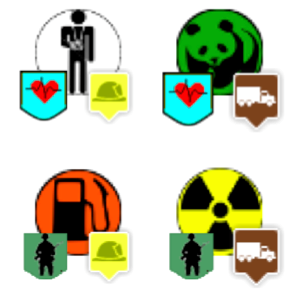
\includegraphics[width=0.3\textwidth]{img/approach/roleTargetMapping}
  \caption{Role-target mapping}
  \label{fig:roleTargetMapping}
\end{figure}

The role-target mapping mechanic requires players to engage in resource coordination. Field responders have to engage in `agile teaming' forming, disbanding, relocating and re-forming in teams over the course of the game in order to complete the game objective. \\

\textbf{The radioactive cloud}. The cloud is a danger zone that can incapacitate field responders. It imposes spatial and temporal constraints on task performance and well- being. The cloud is analogous to various spatial phenomena in disasters (e.g. spreading fires, diseases and floods). It requires communication between HQ and field responders, as the spatial position and movement of the cloud is only known to HQ. The cloud is shown in a heatmap style in the figure \ref{fig:cloud}. The field player can detect `radioactive intensity' at their current locations with the mobile responder app.\\

\begin{figure}[h]
  \centering
  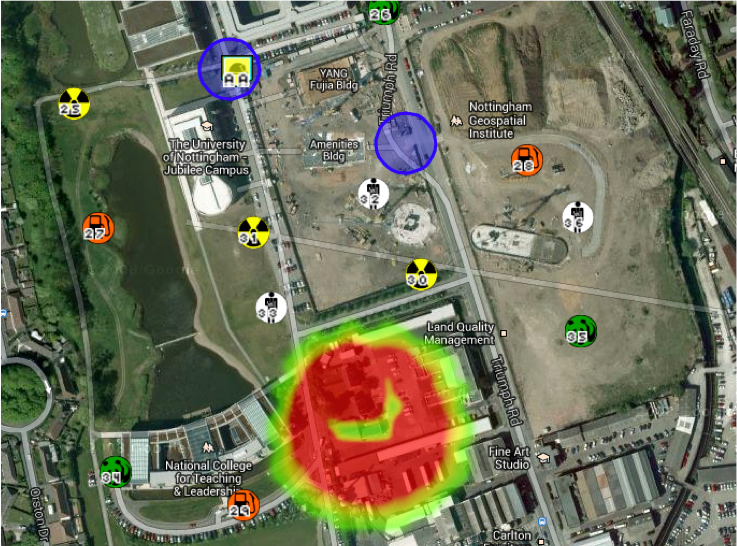
\includegraphics[width=0.8\textwidth]{img/approach/radioactiveCloud}
  \caption{The radioactive cloud}
  \label{fig:cloud}
\end{figure}

\textbf{Command-and-control (C2) structure}. The division of responsibility into HQ and field responders simulates a situation where  responders are connected to a generic two level \ac{C2} structure proposed by \cite{Chen2005}. This structure highlight the division between remote control room and on-site teams.  On-site responders react to the immediate scene without global picture, while the coordination center deals with strategic issues and works with a global picture, leveraging external resources to help on-site response (Section\ref{sec:LRC2}). Instead of simulating a real command and control model such as \ac{BSG} (Section \ref{sec:lrstructure}), we chose the generic structure to simplify the game play, but to still mirror the main characteristics of \ac{C2} in \ac{DR}. \\

\textbf{System interface}. The system interface design is closely related to specific interaction designs, and it is refined through three iterations of field trials. Therefore, the details of interface evolution are left to be introduced in the subsequent chapters (Chapters \ref{ch:studyone},\ref{ch:studytwo},\ref{ch:studythree}) describing field trials. \\



\subsection{System architecture}
The AtomicOrchid system is based on the open-sourced geo-fencing game MapAttack \footnote{http://mapattack.org/} that has been iteratively developed for a responsive, (relatively) scalable experience. Our mixed-reality game relies especially on real-time data streaming between client and server. The client-server architecture is depicted in figure \ref{fig:sysArchitecture}. Client-side requests for less dynamic content use HTTP. Game status and logic is stored and maintained on game server (Appendix \ref{app:datamodel}). Frequent events, such as location updates and radiation exposure, are streamed to clients using websockets to avoid the overhead of HTTP. In this way, field responders are kept informed in near real-time (Appendix \ref{app:architecture}).  \\

\begin{figure}[h]
  \centering
  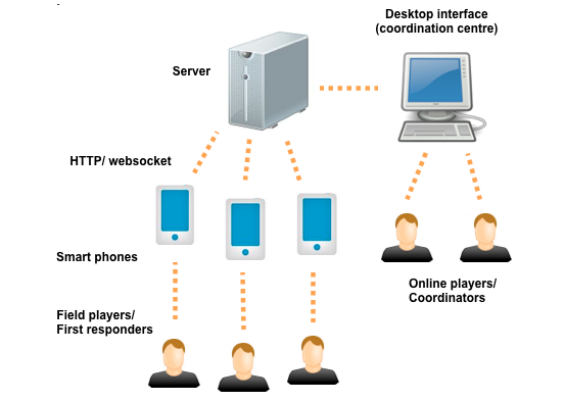
\includegraphics[width=1\textwidth]{img/approach/systemArchitecture}
  \caption{System architecture}
  \label{fig:sysArchitecture}
\end{figure}

The platform is built using Sinatra for Ruby (http://www.sinatrarb.com/), and current web technologies such as socket.io, node.js, and AngularJs, and the Google Maps API. Open source mobile client apps exist for iPhone and Android; we adapted an Android app to build the Mobile Responder App.\\


\subsection{The planning agent}\label{sec:appagent}
In studies 2 and 3 (chapters \ref{ch:studytwo} and \ref{ch:studythree}), planning agents are integrated into AtomicOrchid to support player's planning activities. The agents are developed by ORCHID research partners from Southampton, more technical details of the planning agent is available in \cite{Ramchurn2015a}. In what follows, we briefly describe technical details of the agents and system integration between \ac{AO} and the agents.  \\

The coordination problem (described in section \ref{sec:gameRatinale}) is modelled using a Multi-Agent Markov Decision Process (MMDP) that captures the uncertainties of task execution, extending earlier work \citep{Wu2015}. The model allows responder actions to be delayed or to fail during the rescue process. The MMDP modelling leads to a large search space, even with a small problem. Hence,  an approximate solution is devised to save computation time, which can be executed to support real time planning. The planning algorithm takes into account both time (cloud and human movement speed) and spatial (path planning for responders) constraints. The planning algorithm run by the planning agent produces high quality task allocations that minimise the travelling distance of first responders, and maximise the number of targets rescued. Before the agent was deployed to support human teams in the game setting, computational simulations were used to benchmark the MMDP algorithm against greedy and myopic methods (see figure \ref{tab:agentBenchmarking}). The results confirm that the algorithm produces efficient task allocations.\\


\begin{table}[h]
\centering
\begin{tabular}{c|lll}
Metrics               & MMDP  & myopic & greedy \\ \hline
\#completed task      & 71\%  & 65\%   & 41\%   \\
\#responders survived & 100\% & 25\%   & 0\%   
\end{tabular}
\caption{Result for MMDP, Myopic and Greedy algorithms, Credit \cite{Ramchurn2015a}}
\label{tab:agentBenchmarking}
\end{table}

For integration, the agent is deployed on a separate server. It communicates with the \ac{AO} game server through a pre-defined HTTP protocol (Appendix \ref{app:asprotocel}). The agent takes the game status from the game server as input, which includes player's health, road connectivity, locations of players, targets and radioactive clouds. The output of the agent is a set of task assignments such as `player A and player B, go to target 1' (Figure \ref{fig:inputoutput}) . The task assignments are sent to the \ac{AO} game server and presented to the game players. Detailed interaction design between human and the agent will be presented in Chapter \ref{ch:studytwo} and \ref{ch:studythree}. In order to facilitate the different interaction designs, the input of the agent is slightly different in study 2 and study 3, which will be detailed in sections \ref{sec:studyoneagent} and \ref{sec:studytwoagent}. \\

\begin{figure}[h]
  \centering
  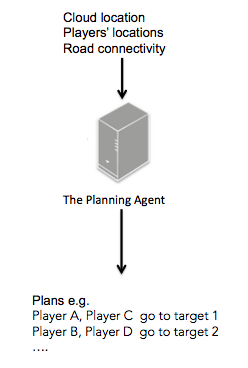
\includegraphics[width=0.5\textwidth]{img/approach/inputoutput}
  \caption{Input and output of the agents}
  \label{fig:inputoutput}
\end{figure}

\subsection{Logging system} \label{sec:applogging}
A logging system is also built into the AtomicOrchid system. The updates of game status sent between the game server and clients (both HQ and mobile clients) are all recorded in JSON format with system timestamps. The logs also contain the information of cloud status, task location and status (pick up/ drop off), messages, player location and health. Automated tools were also developed to reconstruct game play and visualise (Section \ref{sec:methdatahandling}) the log for data analysis. %The detailed log format is documented in Appendix x.

\subsection{Iterative design and development}
Before the game was deployed for observational studies in this PhD work, the game went through an iterative design and development process to test, refine game concepts and system robustness. We briefly describe three cycles of iterative game design and evaluation that took place before the system was ready for the first formal field study.\\

In the first iteration, we used a paper-based prototype to test and refine the core game mechanics. We recruited 12 participants, allocated one of four roles to them, and equipped them only with paper maps with locations of targets. They had to form different kinds of teams to retrieve the different kinds of boxes placed in the game area. The paper prototype demonstrated the demand for better support of situation awareness and communication to enable coordination. The resulting technology prototype was first tested with users in the second iteration. Users were equipped with the responder smartphone app to communicate, navigate, locate and pick up targets in teams formed according to role requirements. HQ was staffed by members of the research team. A pilot study was conducted with members of the public that visited an Open Day at a local university. A total of 20 members of the public tested the game in four ad-hoc game trials. The lessons learned in the pilot study revealed problems with user interaction, networking, and game parameter tuning, which we subsequently addressed.\\

In the third iteration, we improved system stability and interface design. We conducted a pilot study at the campus of another university, to test the system in place. The first full-fledged studies we report on in chapters \ref{ch:studyone}, \ref{ch:studytwo}, and \ref{ch:studythree} were conducted shortly thereafter.\\


\section{Exploring interaction designs with three AtomicOrchid studies}\label{sec:patterns} \label{sec:approachPatterns}

%[Justify the relation between the three iterations]
%- avoiding pitfalls that undermines observation of interaction arrangement
%- HQ agent interaction can be parallel/ HQ FR interaction follows progressive design interaction
%- The first iteraction: base case/ need to understand the organization before we do anything.\\

Based on the serious game approach, three studies have been planned to explore the interactional issues related to the socio-technical integration of the planning agents and the responder team. To build such a socio-technical system, there are various ways to arrange the interaction between responder teams and a planning support agent. Inspired by the \acf{LoA} concept (Section\ref{sec:lrloa}) from research on automation design, we outlined 4 paradigms of human agent interaction loosely based on the automation level of planning activities: full manual, human in-the-loop, human on-the-loop, and Human-out-of-loop. This PhD work will only consider the former 3 notions of automation as explained before\\

In research of automation design, the \ac{LoA} model has been developed to categorise systems into a linear spectrum according to degree of automation. Arguably, the model may not fit perfectly into the context of socio-technical system due to some of its limitations identified in section \ref{sec:lrloa}. However, the terminologies that come with the model can still serve as a reference point for interaction designs to be studied in this PhD work.

%There are several variations of the LOA models. One example is the two-dimensional LOA model proposed by Parasuraman (detailed in literature review section x).Several limitations of the LOA has been identified in chapter x. Most importantly, the LOA model has a focus on one-to-one operator-system interaction (e.g. autopilots, tele-oportation). It fails to capture complexity of the interactions in the context of technology support for organisational work. Therefore, it does not fit into the context of socio-technical system, which is the main focus of this research. 

\begin{enumerate}
\item \textbf{Human out-of-the-loop}.
Out-of-the-loop represents the highest level of automation. An out-of-the-loop system is supposed to run completely independently. The human is replaced by the machine, therefore no human system interaction is required. This is unlikely to be realized in a socio-technical system, in which organisational work is mainly carried out by humans and supported by technologies.  \\

\item \textbf{Human on-the-loop}.
In this research we use the term Human On-the-loop to describe a system with high level of automation, which requires a minimum level of human intervention. Compared to out-of-the-loop, the on-the-loop system is designed to run without human intervention most of the times. However, human supervision and intervention are still required for contingencies. 

\item \textbf{Human in-the-loop}.
In this research human in-the-loop represents a system with medium level of automation. Compared to the on-the-loop system, the in-the-Loop system can not run without human input. Constant human interactions are required to achieve the goal of the socio-technical system. \\

\item \textbf{Full manual}.
A full manual system describes a system without automation. In the context of AtomicOrchid, the platform without integration of the planning agent can be seen as a full manual system. 

\end{enumerate}

In the context of the AtomicOrchid platform, the notions of In-the-loop and On-the-loop can be used to describe the degree to which the planning agent automates the real-time task planning and the extent to which the human Headquarters need to be involved in the plan-execution loop. Guided by these 2 notions, we devised two detailed interaction designs for integrating the planning agent into the \ac{AO} game. In the next two sections, we give detailed description of the two interaction designs, followed up by an overview of the three field studies, which details how a sequence of system prototyping  and field trials was organised based on the two interaction designs, and how they are designed to serve the research objectives.\\

\subsection{The on-the-loop interaction}
The On-the-loop interaction is designed to facilitate the division of labour between humans and agent: a planning agent routinely assigns tasks to distributed responder teams, while human coordinators (the HQ) monitor and support the task execution by responding to arising contingencies (see figure \ref{fig:OnTheLoop}). In this design, the agent can directly contact field responders to allocate tasks. The responsibility of the planning agent is to generate and distribute plans for execution. The agent is also responsible for initiating re-planning according to changes in game status. The agent also directly handles feedback from the field player, i.e. the field players can give feedback to the agent by accepting or rejecting the plan, while the agent can generate new plans according to the feedback. \\

The role of the HQ is to monitor the planning process and provide support when contingencies arise. For example, the HQ may decide to stop some tasks issued by the agent if the threat of radiation increases unexpectedly. It should be noted that the agent can operate without HQ input, and the HQ intervention is supposed to be only occasional. \\

\begin{figure}[h]
  \centering
  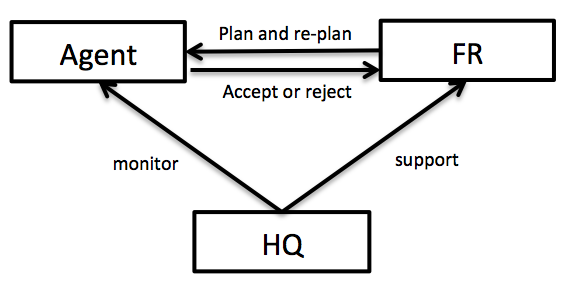
\includegraphics[width=0.5\textwidth]{img/approach/OnTheLoop}
  \caption{On-the-loop interaction design}
  \label{fig:OnTheLoop}
\end{figure}

\subsection{The in-the-loop interaction}
In-the-loop interaction is designed to facilitate a different pattern of labour division between humans and agent: a planning agent proposes the task assignments, and the human HQ needs to approve the tasks before they are sent to the field responders. In this design, the HQ can be seen as a mediator between field responder and the planning agent. If the HQ does not agree with a task allocations from agents, they can intervene by directly editing part of the plan or require the agent to re-plan. \\

Similarly, the feedback from the field responders (i.e. accept/reject) are delivered to HQ before any actions are taken. The HQ are responsible for reviewing the feedback and deciding what actions to take (e.g. decide to initiate re-plan, or ignore). Compared to On-the-loop interaction, the agent in this design will never directly communicate with field responders and the agent cannot operate without the HQ's input, i.e. the HQ have to make decisions on every agent proposed task, and take actions on the feedback from field responders. \\

\begin{figure}[h]
  \centering
  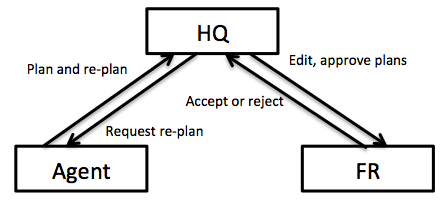
\includegraphics[width=0.5\textwidth]{img/approach/InTheLoop}
  \caption{In-the-loop interaction design}
  \label{fig:InTheLoop}
\end{figure}


\subsection{The three AO game studies}
Three studies are conducted to explore the socio-technical issues related to human-agent interaction. The first study focuses on a ``manual'' version of AtomicOrchid without agent support, while the latter two studies focus on on-the-loop and in-the-loop planning support respectively. For each study, we facilitate several \acf{MRG} sessions to study the interaction design paradigms. \\ 

The first study aims to observe and explore human coordination without planning agent support. The non-agent trial (Chapter \ref{ch:studyone}) supports the two later (Chapter \ref{ch:studytwo}, \ref{ch:studythree}) agent-supported system trials by 1) revealing baseline performance of human coordination without agent support 2) and generating design requirements which feed into subsequent prototyping of AtomicOrchid. The purpose of the second and third studies is to investigate socio-technical issues related to the On-the-loop and In-the-loop interactions and derive design implications of interaction designs from the field observations.\\

\section{Collaboration with a professional Disaster Response organisation}\label{sec:rg}
In addition to the three observational studies of AtomicOrchid games, a workshop with Rescue Global (a professional disaster response agency, see section \ref{sec:rg}) was organised to get professional feedback about the AtomicOrchid system and the planning support agent. Because the contact with Rescue Global was established at a late stage of this PhD work, the feedback from the \ac{RG} workshop are not used to drive the development of \ac{AO} game and interaction design, but to get an insight into the similarities and differences between \ac{AO} simulation and real world \ac{DR} operations, which help us to understand limitations and strengths of our observational study. The in-the-loop \ac{AO} probe was demonstrated to the \ac{RG} team and a discussion was organised to get feedback from \ac{RG}. It included a hands-on session for \ac{RG} members to experience the \ac{AO} game, and further feedback was collected from discussions during and after the game session.\\

\subsection{Introduction of Rescue Global}
\acf{RG} is a disaster response organisation. They are a UK charity and a US not-for-profit headquartered in London, UK. Their remit is to provide ``immediate crisis and disaster reconnaissance ability, delivering accurate and timely information and risk data, as well as performing emergency search and rescue operations where needed to save life.'' One example of their operation is the deployment of a reconnaissance team in the Philippines for super typhoon Haiyan in 2013. After the typhoon strike, the team conducted disaster reconnaissance on isolated islands from the air and on the ground, assessing needs and delivering aid based on priorities of water, food, medicine and shelter.\\

\ac{RG}`s organisational structure represents a typical hierarchy found in emergency services \citep{U.S.DepartmentofHomelandSecurity2008}, termed Gold, Silver and Bronze. Gold denotes the strategic lead, which is associated with \ac{RG}`s senior officers (Section \ref{sec:lrstructure}) and the headquarters in London, Silver is the tactical lead, which is `spun up' for mission planning, both to assess feasibility of deployments and when actually deployed on-site. Bronze refers to the operational level, in which `Pathfinders' (field responders) carry out operations `on the ground' supported by Silver command \citep{RescueGlobal2012}. \ac{RG}`s core staff consists of around 20 highly specialised experts and admin support, many of whom have had prior careers in the military, emergency and first response services.\\

%\section{A framework of interactional issues}\label{sec:interactional}
%interaction techniques 
%[Which Interaction Technique Works When] refer to interaction techniques may refer to is a set of %interface widget design.

%We follows a process of interaction design documented in the [Designing interactions p 15], the process %is interactive, with a special focus on understanding issues and generating design implications . The %issues emerges in previous iterations will be feedback to next iterations. 

%interactional issues: 

%Interface aspects: tech dependent or not?
%interaction aspects: concerned with interaction patterns 
%Social aspects: Corncerned with what? 

%(Sedig, K.Parsons, P) pattern based approach.
%(Most interaction techniques literature reviewed so far is about study in visual representation. )
%(Interaction design, wiki)

\chapter{Methodology to Investigate Human-Agent Interaction}\label{ch:methodology}
This chapter takes an in-depth look at the methodology that underlies the empirical approach adopted in the presented studies. This PhD is based on ethnomethodology oriented field studies based on the \acf{AO} platform to generate descriptive results, which contains rich interactions among participants and the planning support system. Ethnographic observations and interaction analysis are central to all three field studies, while group interviews, message classification, and system log analysis supplement the two former in-situ methods.\\

\section{Ethnomethodological perspective}
Observation of participants in the field study is informed by \acf{EM}. Following the tradition of ethnography, \ac{EM} seeks to explicate the real-world organisation of work by adopting a naturalistic stance. \ac{EM} places methodological emphasis on rigorous description of the situated (i.e. local, observable) actions and practices \citep{Suchman1987} in and through the contingent accomplishment of daily activities. \ac{EM}-informed ethnography arguably helps to answer what might be regarded as an essential question in design: what to automate and what to leave to human skill, competence, judgement, experience and expertise \citep{Crabtree2012}. By producing description of the actions and practices in and through which the work `gets done' time and time again by the members, \ac{EM} can inform system design by uncovering what actions and activities we should therefore support.\\

For the purpose of this thesis, the social situation of the interaction with and around the planning support is argued to be a critical factor to understand how the social organisation of work is achieved. Observation of the situated actions and practice employed by the participants is a key method for the field study. The use of the system was observed and filmed for later analysis. Video is widely recognised as an important resource for ethnography around technology use \citep{Crabtree2012}. The next section goes through the method of video-based interaction analysis for unpacking the interactions observed in the field. \\

\section{Interaction analysis} \label{sec:aprIA}
Interaction analysis can be defined as an interdisciplinary method for empirical investigation of interaction of human beings with each other and with objects in their environments \citep{Jordan1995}. In the context of \ac{HCI} study, it is a method of analysing naturally occurring talk and activity, with the aim of uncovering and describing something of the order and organisation by which people interpret and interact with each other and with the things around them.\\

The advantage of interaction analysis lies in its ability to deal with actual details of technologically mediated interactions and allows technology developers to see exactly how technology fits (or doesn't fit) into current working practice. Other methods such as questionnaires and interviews rely upon reports from participants, rather than actual, reasoning and behaviour. The over-reliance on participants' report make those methods vulnerable to the problems of people producing post-hoc rationalisations of actions, forgetting or incorrectly estimating aspects of behaviour, expressing ineffective attitudes, and generally lacking insight into the tacit procedures underlying much of their activity. Instead, interaction analysis can expose the practical reasoning activities of participant's themselves in a way which does not require them having to remember, justify or even know what they did. This effectively indicates how people think and make sense of technology they are using, in the performance of some task. However, interaction analysis is extremely time-consuming, which means it can only be carried out on small numbers of participants. This limitation makes it unsuitable for answering to very specific design questions and for examining the needs and behaviours of diverse groups of people. Further, the generality of its findings may need to be established by other means \citep{Jordan1995}.\\

For the purpose of this PhD work, interaction analysis is applied to the observations of the game probes undergoing field trials. In this case, the description generated by interaction analysis could expose information on the sequential organisation of technologically and socially mediated activities, which in turn, reveals how the activities can be supported. The main resource of interaction analysis is video recordings of \ac{AO} game plays. The video analysis generally consists of three stages \citep{Heath2010} :

\begin{enumerate}

\item Cataloguing the data corpus. This step involves a preliminary review of the corpus. Basic aspects of the activities and events are catalogued at this stage. Preliminary reviews and cataloguing should involve no more than a simple description and classification of the materials without detailed analysis. \\

\item Selecting Episodes. In light of preliminary review of data, a more focused substantive review of data is carried out in this stage. Repeated analytical searches of the data corpus are also involved to find examples of actions that appear to reflect similar characteristics. Candidate episodes of the particular phenomena, actions or organisation under scrutiny should be gathered and put into collections. \\

\item Detailed analysis.  We begin to look more closely at the selected candidate episodes to unpack the way in which interaction is accomplished by participants. The process generally involves transcribing and analysing both talk and visible conduct in the candidate episodes. \\ 

\end{enumerate}

In the later chapters, results of interaction analysis are presented in detailed episodes of game play. In those episodes, a standard orthographic notation is used \citep{Jordan1995} and complemented by timestamps [0:00], and system messages from remote players and HQ. Players can be uniquely identified by their initials. Targets are denoted by their unique numeric target id. Task assignments from the planner support system are represented as two initials and one target id connected by a rightward arrow. For example, the notation PC, CR -> 22 means player PC and CR are instructed to team up and go for target 22.\\




\section{Data collection and handling}\label{sec:methdatahandling}
Interaction analysis has been introduced as the main method for investigating socio-technical issues in our studies. This section introduces a number of methods employed for data collection and handling. In particular, the group interview supplements field observation by providing subjective description of game play experience. The message classification method gives quantitative overview of remote communication. It also provides context for interactions in the field and helps to identify interesting game events. The system log analysis produces game event visualisations and replay. When triangulated with the video data, the log data analysis also supports interaction analysis by providing context and helping to identify interesting episodes in videos.\\

\subsection{Video and audio recording}
Audio recorders and video cameras are believed to valuable resources for ethnographic study. Both audio and video recordings offer us a rich resource and enable us to elucidate the methodical ways in which work is organised and accomplished as an interactional matter \citep{Crabtree2012}. This PhD work uses video/audio recordings to capture distributed activities in the \acf{AO} game as it happens, and the subsequent interaction analysis is based on reviewing the video recordings. \\

For each \ac{AO} study, multiple researchers were hired to capture activities of distributed teams in the field. The researchers were instructed to follow player teams and film their actions including talking, gestures, and other bodily activities. In some cases, there weren't enough researchers to cover all the player teams in the field. To maximise the number of teams covered, the researchers were instructed to avoid filming the same player teams at the same time. In the control room, one researcher recorded the actions of Headquarters players with two camcorders. One camcorder was fixed on a tripod and the other was held by the researcher. \\

Audio recordings were used to supplement videos. An audio recording app was installed in the Android phones that were used by the field players in the \ac{AO} game. The app works in the background, recording player's voices without interrupting players' use of the AtomicOrchid client app. The obvious limitation of audio is that we cannot visually see player's actions with it, while its strength lies in its guaranteed coverage of all player teams at all times. As a great deal of the work of a setting is conducted through talk \citep{Crabtree2012}, audio recordings are useful alternative resources for interaction analysis when video coverage is not sufficient. \\


\subsection{Log data handling} \label{sec:aprloghandling}
\acf{HCI} researchers often collect rich dataset for investigating interactions. The data set becomes larger and larger as digital record systems increase in availability \citep{Brundell}. Automated tools are increasingly necessary for managing the organisation, replaying, structured and free coding (and annotation) and analysis of these growing data sets \citep{Brundell}. For this research, the logging system of AtomicOrchid produces time-stamped system logs. The raw log data is hard to be used directly as a resource for interaction analysis. In order to reveal the information buried in the logs, the data has to be processed so that it can be easily read and triangulated with data in other modalities i.e.  video and audio recordings. There are a number of tools already in existence to automate data handling and support the analysis of interactions. However, these tools often have limited or very specific functionalities \citep{Brundell}. Therefore, we developed our own data visualisation and log replay system which are tailored to handle the raw log data from the AtomicOrchid studies.\\

To recap (Section \ref{sec:applogging}), the logging system records players's location, health, targets' location and status (pick up/drop off), task assignments and players' feedback (reject/accept). The data visualisation tool (Figure \ref{fig:logvis}) focus on visualising task assignments in the game play. The game events related to task allocations, including task assignments, player feedback, target pickup and dropoff, are all plotted on a time line with different annotations. The colored dots and squares denote various game events (Figure \ref{fig:logvis}). Detailed information of the event can be displayed when mouse hover on. As can be seen in Figure \ref{fig:logvis}, the deep blue dot with mouse cursor hover on denotes a target pick up event. The two players with initials CY and DS (see lines connecting the pick-up events) picked up target 598 at the 10th minute of game play. This data visualisation tools give an overview of the game-event sequence. It assists interaction analysis by providing context and guidance in the episode selection process. \\

\begin{figure}[h]
  \centering
  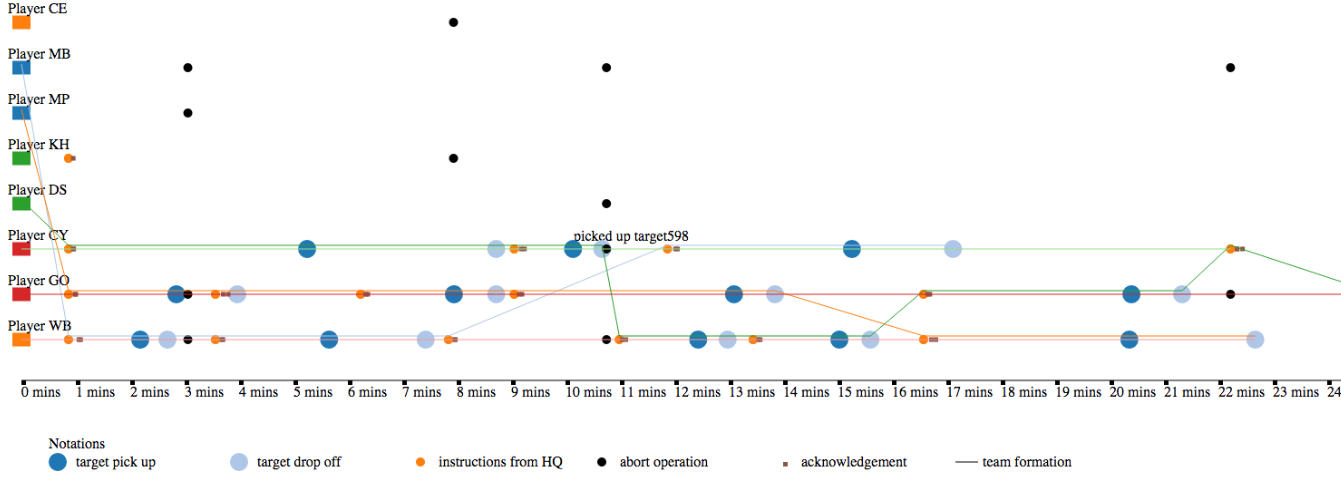
\includegraphics[width=1\textwidth]{img/methodology/logVisualisation}
  \caption{Log visualisation}
  \label{fig:logvis}
\end{figure}

A replay system was also built to triangulate multiple videos with log data. The main map view on the replay interface (Figure \ref{fig:replay}) displays game status reconstructed from log data, in a way that is similar to the HQ interface. By giving a time offset to each video file, the videos are synchronised with the main map view of game status. The replay system is an important tool for interaction analysis, as it presents distributed game play within a single interface in a synchronised way, providing insights into the distributed interaction among participants and the system as it happened in parallel. \\

\begin{figure}[H]
  \centering
 \rotatebox{90}{
  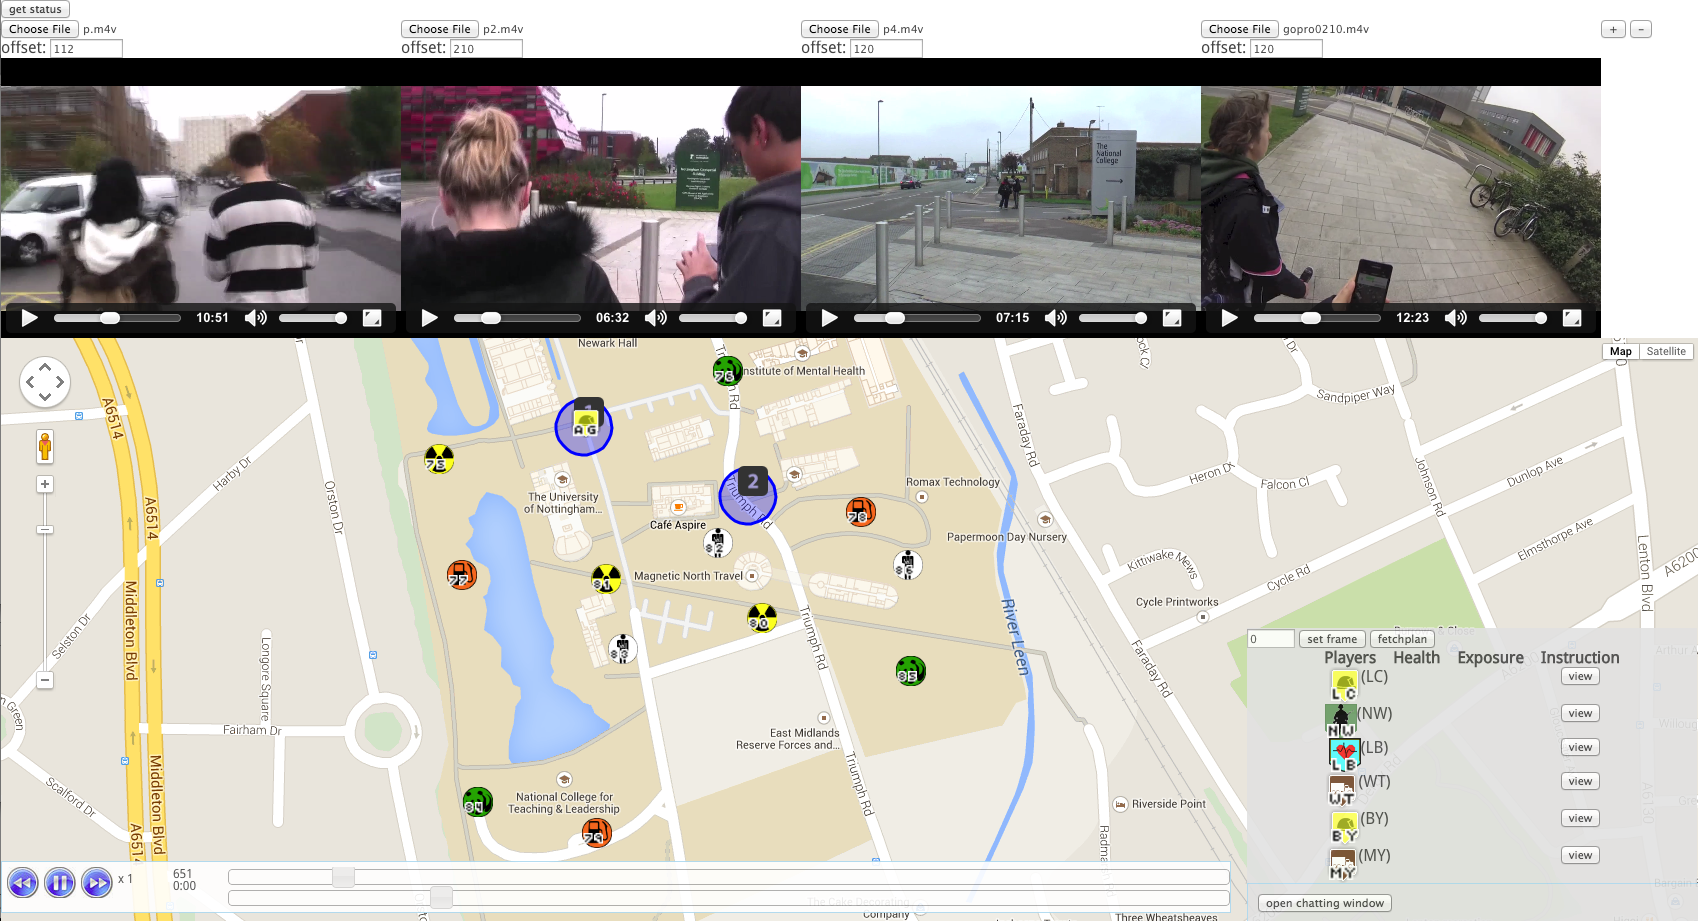
\includegraphics[width=1.5\textwidth]{img/methodology/replay}
 }
  
   \caption{Replay system}
  \label{fig:replay}
\end{figure}
\newpage
\subsection{Message classification} \label{sec:aprmsg}
In AtomicOrchid, remote coordination between field and human HQ is achieved through a text messaging channel. The remote messages are recorded as part of system logs. To understand how the team members interact through the remote messages, we devised a message classification method based on speech act theory \citep{Searle1976}. We used speech-act theory and the notion of adjacency pairs \citep{Avrahami} to classify messages sent between and among responders and HQ. According to speech act theory, utterances in dialogues can be considered as speech acts from three dimensions \citep{Searle1976}. We were primarily concerned with the illocutionary dimension of speech acts.\\

Searle`s classification of illocutionary acts is used to categorize messages in the communication system as follows.\\

\begin{enumerate}
\item Assertives: speech acts that commit a speaker to the truth of the expressed proposition.
\item Directives: speech acts that are meant to cause the hearer to take a particular action, e.g. requests, commands and advice.
\item Commissives: speech acts that commit a speaker to some future action, e.g. promises and oaths.
\item Expressives: speech acts that express the speaker's attitudes and emotions towards the proposition, e.g. congratulations, apologies and thanks.
\item Declarations: speech acts that change the reality in accord with the proposition of the declaration, e.g. pronouncing someone guilty.
\end{enumerate}

The notion of request-response adjacency pairs are also used to gain insights into the reciprocity of communication. In linguistics, adjacency pairs describe conversational turn taking \citep{Avrahami}. In AtomicOrchid, we expected many actions in remote conversation to be accomplished through pairs of utterances such as request-response, question-answer, or inform-acknowledge. For simplicity, we ignore the typology of adjacency pairs and treat all pairs as request-> response. Any utterance that expects a response is considered as a request.\\

The purpose of this message classification is to give an overview of the communication in the message channel. Meanwhile, the results of message classification supports interaction analysis, as it helps to identify interesting moments of team interaction in the game such as important decision points.\\

\subsection{Group interview}
For all three field studies, group interviews were conducted with all participants after each game sessions. The interviews consist of open-ended questions with the aim to supplement the field observation and interaction analysis with participants' comments about their experiences of the game. The interview is `informal and unstructured' in the sense that it is not driven by pre-defined questions, but only by the research scope and interest. It is conducted in the manner of a conversation taking place between the researcher and the participants \citep{Crabtree2012}. The interview does not stand on its own to provide distinctive results. The primary aim of the interview is to develop an overview of participants' experience of the game. Meanwhile, emergence of unanticipated issues and events was also fostered by asking open-ended questions, which in turn, are used to establish context for the issues for interaction analysis.\\

\section{Analytic procedure}
To sum up, interaction analysis is the main analytic method applied in the studies. The data collection and handling processes are supported by methods including log data handling, group interviews and message classification. With this inventory of research methods, we can depict a typical analytic procedure for analysing the interactions in as AtomicOrchid study. \\

The procedure (Figure \ref{fig:analyticprocedure}) begins with field studies after which a set of data are collected from three sources including system logs (1.1), video/audio recording (1.2) and group interviews (1.3). The message logs are then classified according to speech act theory. The resulting classification gives quantitative insight into the remote communication. The further log data handling produces replay and visualisation of game events. \\

The outputs of the data handling process are then used as resources for interaction analysis. The message classification (2.1) contribute to the catalogue building process (3.1) in the interaction analysis by providing the context of remote communication. The data visualisation (2.2) also helps to identify important episodes of interaction and provide context for further episode analysis. The game replay (2.2) triangulate video recordings with system logs. It is used as the major tool for in-depth data examination in the episode selection and analysis process (3.2,3.3), as it provides a synchronised view of multiple videos and system logs. Additionally, the players' comments from the group interview give us insights into participants' subjective game experience, which provides further context for episode analysis.\\



\begin{figure}[h]
  \centering
  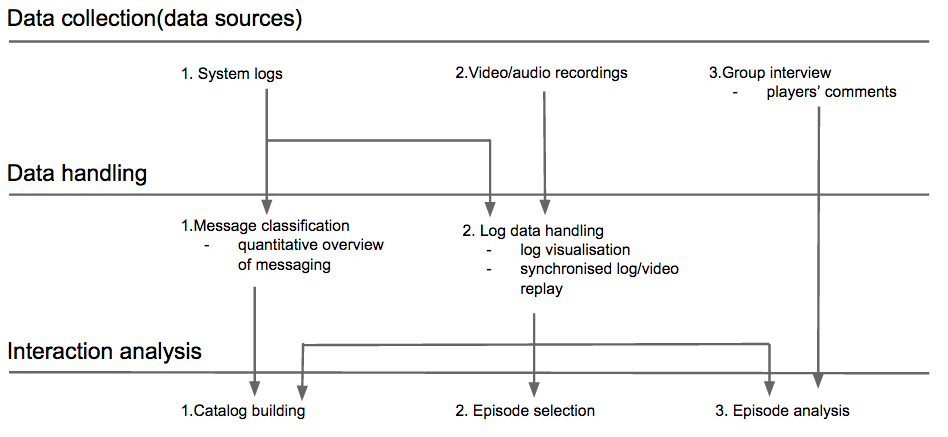
\includegraphics[width=1\textwidth]{img/methodology/analyticprocedure}
  \caption{Analytic procedure}
  \label{fig:analyticprocedure}
\end{figure}

